% arara: pdflatex: { shell: yes }
% arara: biber
% arara: pdflatex: { shell: yes }
% arara: pdflatex: { shell: yes }

% Demo report and presentation prepared by Aaron English (humdrumcomet on github)
\documentclass[hidelinks, 12pt]{article}%

\usepackage{geometry} % useful for defining page geometries
\usepackage{hyperref} % used for creating hyperlinks in documents. Both to the web and within the document itself
\usepackage[tbtags]{amsmath} % for typesetting math (American Mathematical Society)
\usepackage{amsfonts} % fonts and mathematical symbols
\usepackage{amssymb} % more mathematical symbols
\usepackage[utf8]{inputenc} % how to treat the written file (as utf8)
\usepackage[T1]{fontenc} % the encoding for the output file T1 is the most common, includes accents and many other commonly needed/used characters
\usepackage[style=ieee,backend=biber]{biblatex} % for handling bibliographies
\usepackage{float} % added control over floats
\usepackage{graphicx} % tools for inclusion of graphics
\usepackage{csvsimple-l3} % simplify table creation by importing .csv files directly (the l3 version is the current most up-to-date version of the package)
\usepackage{tabularray} % The current best and most modern tables package available
\usepackage{booktabs} % generate publication ready tables
\usepackage{siunitx} % consistent notation and correct formatting of units
\UseTblrLibrary{booktabs, siunitx, amsmath, diagbox} % Incorporating in other desirable features for ease of table formatting
% Configuring the siunitx package
\sisetup{
detect-family = true,
detect-weight = true,
per-mode = reciprocal,
input-digits = { 0123456789\pi\dots },
input-comparators = { <=>\approx\ge\geq\gg\le\leq\ll\sim\gtrsim\lesssim },
table-figures-integer = 3,
table-figures-decimal = 2,
table-auto-round,
}%
\DeclareSIUnit\torr{Torr} % Custom unit definition
\usepackage{minted} % inclusion of code blocks with syntax highlighting and
\setminted{linenos, autogobble, fontsize=\footnotesize, breaklines=true} % set global options for minted environments
\usepackage{chemformula} % for writing chemical formulae
\usepackage[useregional]{datetime2}

\addbibresource[location=local]{references.bib} % adding a bibliography

\begin{document}
    \begin{center}
        \vspace*{1cm}
        {\fontsize{300}{50}\selectfont {\bfseries Hello \LaTeX\\}}
        \vspace{3cm}
        {\LARGE An Introduction to the\\
            Typesetting Tool\\}
        \vspace{8cm}
    \end{center}
    \begin{flushright}
        Authors and Organizers:\\
        Ghassan Arnouk\\
        Alec Bales D'Cruze\\
        Aaron English\\
        \DTMdisplaydate{2022}{9}{26}\\
    \end{flushright}
    \thispagestyle{empty}

    \clearpage
    \tableofcontents
    \clearpage
    \section{The Basics}
        \begin{itemize}
            \item environments
                \begin{minted}[linenos=false]{tex}
                    \begin{<environment>}
                        <your code>
                    \end{<environment>}
                \end{minted}
            \item commands
                \begin{minted}[linenos=false]{tex}
                    \command[<some options>]{<arguments>}
                \end{minted}
        \end{itemize}

    \section{Sections...}
        \subsection{...and subsections...}
            \subsubsection{...and subsubsections...}

    \section{Equations}
        How about some equations? An inline equation, showing the Pythagorean theorem \(a^{2} = b^{2} + c^{2}\).
        Or a bigger example, one that I'd like to reference and discuss more, the Fourier Transform as given in Equation \ref{eqt:fourTrans}.
        \begin{equation}
            \hat{f}\left(\xi\right) = \int_{-\infty}^{\infty}f\left(\xi\right)e^{2\pi ix\xi}\text{d}\xi
            \label{eqt:fourTrans}
        \end{equation}
        What if instead I wanted to show substitution and developing equations? (notice the size of the brackets...)
        \begin{align}
            \delta & = B\left(\frac{1}{173} - \frac{B}{180,000}\right) + 0.5\nonumber      \\
                   & = 533\left(\frac{1}{173} - \frac{533}{180,000}\right) + 0.5 \nonumber \\
                   & = 2.0 \nonumber
        \end{align}
        Or even a matrix
        \begin{equation*}
            A =
            \begin{bmatrix}
                -\alpha_f-\beta_1 & 2                 & \frac{1}{c} \\
                -4i               & \sqrt{5-\alpha_f} & -6          \\
                c                 & \beta_1           & 9 + i
            \end{bmatrix}
        \end{equation*}
        A set of differential equations!
        \begin{align}
            \frac{\text{d}x}{\text{d}t} &= \sigma (y-x)\\
            \frac{\text{d}y}{\text{d}t} &= x(\rho -z)-y\\
            \frac{\text{d}z}{\text{d}t} &= xy-\beta z
        \end{align}


    \clearpage
    \section{Figures}
        You can add lovely figures, and then reference them like this "As stated in Figure \ref{fig:test}".
        It's even a hyperlink! \textit{*click* *click*}
        \begin{figure}[H]
            \begin{centering}
                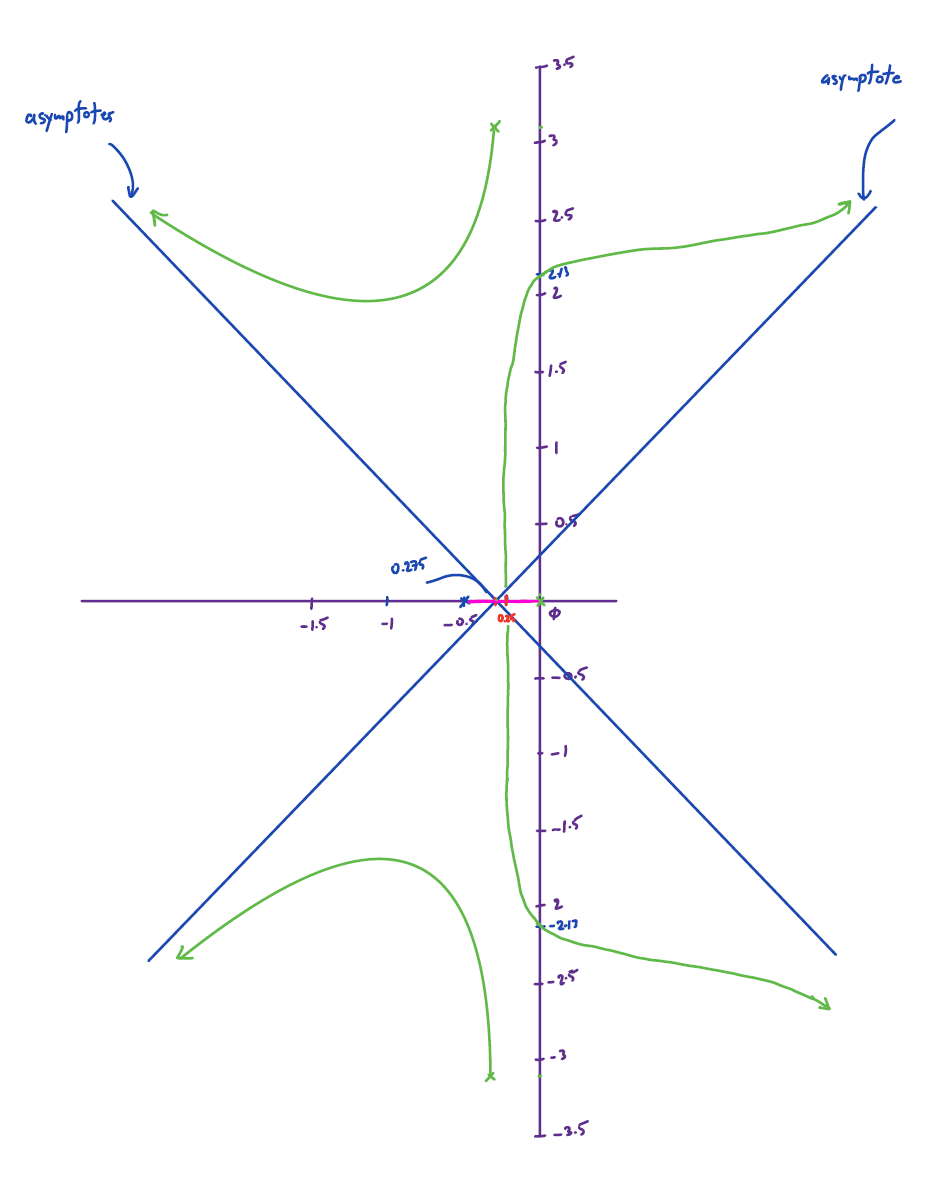
\includegraphics[width=0.5\textwidth]{images/rootLocus.png}
                \caption{A test figure}
                \label{fig:test}
            \end{centering}
        \end{figure}

    \section{Tables}
        What are tables like?
        Like this!
        \begin{table}[H]
            \centering
            \label{Table:Parameters}
            \caption{Table of specified parameters and achieved values}
            \csvreader[
                head to column names,
                centered tabularray = {
                    width=0.9\textwidth,
                    colspec={
                        Q[co=1,l]
                        Q[co=1,c]
                        Q[co=1,c]
                        Q[co=1,c]
                        Q[co=1,c]
                    },
                    row{1} = {guard}
                },
                table head = \toprule \bfseries Parameter & \bfseries Target & \bfseries Calculated & \bfseries Simulated \\\midrule,
                table foot = \bottomrule,
            ]{data/TargetsAndVals.csv}{}{
                \parameter & \tablenum[table-format=<-3.2e1]{\target} & \tablenum[table-format=<-3.2e1]{\theoVal} & \tablenum[table-format=-3.2e1]{\simMixVal}}
        \end{table}

        Add other tables that show just SIunitx
        show multicell

        Can also make use of online table generation tools like \href{https://www.tablesgenerator.com/}{Tables Generator}.

    \section{Bibliographies}
        \subsection{Citations}
            Here I am making a statement that should be backed up with a reference placed right at the end. \cite{ref:01}
            Now it will show up in the bibliography and the reference above will link to it and be correctly numbered.
            Style can be changed at any time up above in the biblatex command.
        \subsection{Writing the .bib File}
            \begin{listing}[H]
                \begin{centering}
                    \begin{minted}{bibtex}
                        @incollection{ref:01,
                        author = {Berger, M.J. and Hubbell, J.H. and Seltzer, S.M. and Chang, J. and Coursey, J.S. and Sukumar, R. and Zucker, D.S. and Olsen, K.},
                        title = {XCOM: Photon Cross Sections Database},
                        publisher = {NIST, PLM, Radiation Physics Division},
                        year = {2010},
                        booktitle = {NIST Standard Reference Database 8 (XGAM)},
                        chapter = {Copper},
                        url = {https://physics.nist.gov/cgi-bin/Xcom/xcom3_1},
                        }
                    \end{minted}
                    \caption{Code for a bibliographic entry}
                    \label{lst:bibliography}
                \end{centering}
            \end{listing}
            While you may have to write a bib entry manually occasional, almost all journal websites offer .bib citations to copy and paste (or download).
            There are also a number of tools that simplify .bib generation:
            \begin{itemize}
                \item Lookup books by their ISBN and get a bibtex entry \href{https://lead.to/amazon/com/?key=+&si=all&op=bt&bn=&so=sa&ht=us}{lead.to}
                \item Browser extension to create bibtex entries from the current webpage (available for firefox and chrome)\href{https://github.com/Langenscheiss/bibitnow}{bibitnow}
                \item many others
            \end{itemize}

    \section{The Power of Open Source}
        \begin{itemize}
            \item Widely available and extraordinarily flexible
            \item Enormous and extremely helpful user base - debugging less of an exercise in pulling teeth
                \begin{itemize}
                    \item \href{https://www.ctan.org/}{CTAN - Comprehensive TeX Archive Network}
                    \item \href{https://tex.stackexchange.com/}{TeX Stack Exchange}
                    \item \href{https://www.overleaf.com/learn}{Overleaf guides}
                \end{itemize}
            \item Continuous extension via community created packages
        \end{itemize}

        \subsection{Recommended Packages}
        \subsubsection{siunitx}
            I strongly recommend using the siunitx package for formatting all units.
            \\\si{\hertz}
            \\\SIrange{100}{200}{\nano\meter}
            \\\SI{100}{\kilo\gram}
            \\Convenient!

        \subsubsection{tabularray}
            The most complete and modern table formatting package.

        \subsubsection{csvsimple}
            Ease preparation of tables by importing csv files directly

        \subsubsection{chemformula}
            A chemical (or nuclear) equation!
            \begin{equation}
                \ch{
                ^{2}H + ^{2}H -> ^{3}He + n^{0}
                }
                \label{eqt:nucEnerReleased}
            \end{equation}

        \subsubsection{minted}
            Include blocks of code or source files with syntax highlighting.
            \begin{listing}[H]
                \inputminted{python}{./demo.py}
                \caption{An example of a block of python included and highlighted with the package minted}
                \label{lst:pythonExample}
            \end{listing}


    \section{As For Modularity and Reusability...}
        \subsection{Preamble Starting Point}
            \begin{minipage}{\textwidth}
                \begin{minipage}{0.4\textwidth}%
                    \begin{enumerate}
                        \item geometry
                        \item hyperref
                        \item amsmath
                        \item amsfonts
                        \item amssymb
                        \item inputenc
                        \item fontenc
                        \item biblatex
                        \item float
                        \item graphicx
                        \item booktabs
                        \item csvsimple
                        \item siunitx
                        \item minted
                        \item chemformula
                    \end{enumerate}
                \end{minipage}
                \begin{minipage}{0.6\textwidth}%
                    \begin{minted}{tex}
                        \usepackage{import}
                        \usepackage{geometry}
                        \usepackage{hyperref}
                        \usepackage[tbtags]{amsmath}
                        \usepackage{amsfonts}
                        \usepackage{amssymb}
                        \usepackage[utf8]{inputenc}
                        \usepackage[T1]{fontenc}
                        \usepackage[style=ieee,backend=biber]{biblatex}
                        \usepackage{float}
                        \usepackage{graphicx}
                        \usepackage{booktabs}
                        \usepackage{csvsimple}
                        \usepackage{siunitx}
                        \usepackage{minted}
                        \usepackage{chemformula}
                    \end{minted}
                \end{minipage}
            \end{minipage}

    \section{What's Next?}
        \begin{itemize}
            \item simplify code reuse? import!
            \item custom graphics and more? PGF/TikZ!
            \item fancy glossaries and acronyms? glossaries!
            \item presentations? beamer!
            \item and still more at the coming workshops!
        \end{itemize}
    \clearpage
    \printbibliography[heading=bibintoc]
\end{document}
